\documentclass[10pt]{article}
\usepackage{tikz}
\usetikzlibrary{arrows}
\usepackage{natbib}
\usepackage{graphicx}
\usepackage{url}
\usepackage{fancyhdr}
\pagestyle{fancy}

\lhead{CAPTools Documentation}
\rhead{KU System-Level Design Group}
\lfoot{\copyright The University of Kansas, 2019}
\cfoot{\thepage}

\newtheorem{conjecture}{Conjecture}
\newtheorem{obligation}{Obligation}
\newtheorem{definition}{Definition}

\usepackage[textsize=tiny]{todonotes}
%%\usepackage{ifthen}
% \newboolean{submission}  %%set to true for the submission version

\newcommand{\squash}{\itemsep=0pt\parskip=0pt}

\parskip=\medskipamount
\parindent=0pt

\bibliographystyle{abbrvnat}


\title{Certified Attestation Protocol Tools - Version 0.1}
\author{Anna Fritz \\
  Information and Telecommunication Technology Center \\
  The University of Kansas \\
  \url{arfritzz@ku.edu}
}

\begin{document}

\section {Initial Overview}

  Negotiation occurs between two parties: the appraiser and the target. The goal is to gather evidence about a target.
  The appraiser sends the target a \textbf{request}. The target then responds
  with a \textbf{proposal} which is a set of \textbf{protocols}.

\section {Basics}

To begin constructing the language, there are basic things we must implement. 

\begin{itemize}
\item Place
	\begin{itemize}
	\squash
	\item Necessary to understand where the Negotiation is taking place.
	\item Maybe place will be specialized for both the appraiser and the target but that is a question for later
	\item For now, place is a natural number that represents where the Negotiation is occurring.  
	\end{itemize}
\item Term
	\begin{itemize}
	\squash
	\item A term is a Copland term. 
	\item This is useful for the Privacy Policy to decide what terms can be shared. 
	\item A Proposal will be composed of a list of terms from the target to the appraiser.
	\item I suppose when we go to define an ordering to establish a meet and join we will order the terms. This seems like a natural place to establish ordering. 
	\end{itemize}
\item Request
	\begin{itemize}
	\item A request asks the target for evidence. 
	\item It can ask for one thing, one thing or the other thing, or both things. 
	\item Request is an Inductive definition then so that the constructors can be `one` `prod` `sum`.
	\end{itemize}
\item Proposal
	\begin{itemize}
	\item Proposal is a definition (function) which takes a request and generates a list of terms
	\item Somewhere somehow the privacy policy must be satisfied. 
	\item Dr. A suggest making a theorem that says "forall protocols, the privacy policy is satisfied"
	\item This leads me to ask "How do we write the privacy policy in terms of code?"
	\end{itemize}

\end{itemize}

Knowing these pieces are needed, an initial step by step procedure can be composed.
\begin{enumerate}
\item A Request is generated from the appraiser and sent to the target
	\begin{itemize}
	
	\end{itemize}
\item The target looks at the proposal and 
\end{enumerate} 

\begin{figure}[hbtp]
  \centering
  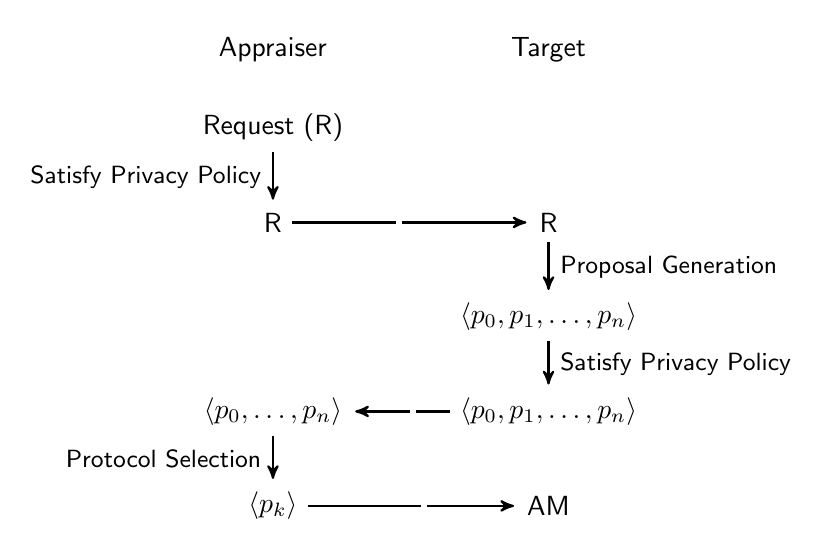
\begin{tikzpicture}[->,>=stealth',shorten >=1pt,auto,node distance=1.2cm,
  thick,main node/.style={rectangle,%%fill=blue!20,draw,
    font=\sffamily,minimum height=2mm,minimum width=2mm}]


  \node[main node] (Request) {Request (R)};
  \node[main node] (AppPrivPol) [below of=Request] {R};
  \node[main node] (R) [node distance=3.5cm, right of=AppPrivPol] {R}; 
  \node[main node] (TarPrivPol) [below of=R] {$\langle p_0,p_1,\ldots,p_n\rangle$}; 
  \node[main node] (TarProp) [below of=TarPrivPol] {$\langle p_0,p_1,\ldots,p_n\rangle$};  
  \node[main node] (AppProp) [node distance=3.5cm, left of=TarProp] {$\langle p_0,\ldots,p_n\rangle$};
  \node[main node] (Protocol) [below of=AppProp] {$\langle p_k\rangle$};
  \node[main node] (AM) [node distance=3.5cm, right of=Protocol] {AM}; 
  \node[main node] (IN) [node distance=1.0cm, above of=Request] {Appraiser};
  \node[main node] (OUT) [node distance=3.5cm, right of=IN] {Target};
    

  \path[every node/.style={font=\sffamily\small, fill=white,inner sep=1pt}]
    (Request) edge node[left=1mm] {Satisfy Privacy Policy} (AppPrivPol)
    (AppPrivPol) edge node[left=1mm] {} (R)
    (R) edge node[right=1mm] {Proposal Generation} (TarPrivPol)
    (TarPrivPol) edge node[right=1mm] {Satisfy Privacy Policy} (TarProp)
    (TarProp) edge node[right=1mm] {} (AppProp)
    (AppProp) edge node[left=1mm] {Protocol Selection} (Protocol)
    (Protocol) edge node[right=1mm] {} (AM)	
	;
\end{tikzpicture}

%%% Local Variables: 
%%% mode: latex
%%% TeX-master: "certification"
%%% End:

  \caption[Attestation and Appraisal Sequence for One Request]{Processing sequence for
    Negotiation, Selection, Attestation and Appraisal during remote
    attestation.}
  \label{fig:att-app-seq}
\end{figure}

\section {Privacy Policy}

At this point, the privacy policy is some large, overarching being that controls the data that is sent back and forth between the appraiser and the target. Both the appraiser and the target have their own, unique privacy policies. Also, in more general terms, each computer or cluster must have a privacy policy as a target and as an appraiser so that it can morph between the two roles. 

\section {Ideal trust establishment function}

The ideal trust establishment $\delta_m:R\rightarrow
(E,\preceq,\top,\bot)$ or delta_m. 

$\delta_m$ relates a request to the set of all evidence packages that 
could result from that request.  Those evidence packages are ordered
by $\preceq$ that defines relative``quality'' of evidence.  If
$e_1\preceq e_2$ then evidence $e_2$ is of higher quality than $e_1$.
Quality is subjective and this order reflects situational awareness.
The relation $\preceq$ is by definition a partial order 
over evidence while $\bot$ and $\top$ are the worst and best evidence
corresponding to no description and an exact description
respectively.  This defines a bounded lattice, however more work is
needed to establish the correctness of the approach.

$\gamma_n$ produces a proposal $\langle p_0,p_1,\ldots,p_n\rangle$
from a request, $r$ based on target policy.\todo{Consider defining
  $\gamma_n$ as a relation and the proposal as the vector of protocols
  for some $r$ as the set of protocols related to $r$.}  $\delta_c$
transforms the proposal into evidence from each protocol,
$\langle e_1,e_2,\ldots,e_n \rangle$. Thus $\delta_c$ is a functor
over proposals---vectors of protocols---to vectors of evidence.
$\alpha_n$ lifts the evidence vector into the evidence lattice.

\section {Request}

\subsection {Certificate Authority}
  
  As part of ISAKMP, a certificate authority is needed for strong 
  authentication of a communicating peer (ie the appraiser and the
  target). 

\subsection {Request Composition}
  
  Right now the exact understanding of the Request is not important.
  Only a general understanding in needed and useful. 
  
  A request is composed of some sort of evidence. It can be three things:
  \begin{enumerate}
  \squash
  \item one evidence
  \item sum of evidence (OR)
  \item product of evidence (AND)
  \end{enumerate}

  
  At this point, there really is not much else that is needed for a Request; all that is needed is evidence. In the future, some things that should be considered in the request are:
  
  \begin{itemize}
   \squash
   \item place
   \item the appraiser privacy policy
   \item ISAKMP
  \end{itemize}

\section {Proposal}

\subsection {Producing a proposal}

  A proposal is a set of protocol generated by the target upon receiving the target's request. Therefore, the proposal takes in the appraiser's request and returns a list of terms. The coq definition for this may look something like an is considered an interpreter: 
  
  \begin{verbatim}
  Definition propose : (request ev) -> list term
  \end{verbatim}  
  
  In this definition, the appraiser receives a list of terms. The list of terms must satisfy the privacy policy for the target before being sent to the appraiser. In the future, some things that should be considered in the proposal are:
  
  \begin{itemize}
   \squash
   \item the target's privacy policy
   \item ISAKMP
  \end{itemize}
  
	I believe that in the proposal, the meet and join should be established. This will make the function of selection a protocol for evaluation easier if the set returned to the target is already ordered. 

\section {Selecting Proposal}

  The function, ($\gamma_{n}$), selects a protocol (P_{k}) 
  from a proposal $\langle p_0,p_1,\ldots,p_n\rangle$.  

  The selection of a Proposal will involve ensuring that the chosen protocol meets the initial negotiation condition. This can be represented in an Inductive definition as follows:
  
  \begin{verbatim}
  Inductive negotiationR : Request -> Place -> term -> Prop :=
  | n1 : (ev1) -> n -> (USM 1) -> True
  .
  .
  .
  . where one can list various options for negotiation. 
  \end{verbatim} 
  
  
  
\section {Evaluating Proposal}

Evaluating a proposal will occur in the Attestation Monad. The job of Negotiation is simply to choose a protocol that will be evaluated. 

\section {How ISAKMP fits} 

In general, ISAKMP is the protocol that establishes Security Associations (SA) and cryptographic keys.It allows an entity's initial communications to indicate which certificate authorities (CAs) it supports.   

\section {Questions:}
\begin{enumerate}
  \item What does the certificate authority get us? A secure channel but 
        does it say anything about the appraiser or target's
        privacy policy?
  \item How does the request generate a proposal? 
  \begin{itemize}
    \item Could think of a request as a condition like all even numbers.
    \item Then Proposal consists of many different sets composed of even
          and odd numbers with each set having varying amounts of numbers.
    \item Then what filters the set to include only even numbers?
          Is that $\delta_c$?
    \item $\delta_c$ is a functor that transforms proposals into evidence.
          I don't really understand this at all.  
  \end{itemize}
  \item Is the targets response, the proposal, an ordered list?
        I think we need a function to ensure ordering.
\end{enumerate}

\section {Examples}

Throughout the process of understanding negotiation, there are many examples that have helped me get a better grasp on Coq and what Negotiation entails. 

\subsection {The Fruit Example: understanding constructing values}

Let Fruit be a set such that Fruit = { apple , orange , pear }. Then an inductive data structure for Fruit could read:  

\begin{verbatim}

Inductive request : Type := 
 | one n -> fruit
 | prod fruit -> fruit -> fruit
 | sum fruit -> fruit -> fruit.
\end{verbatim}

Where prod is equivalent to the boolean condition AND and sum is equivalent to the boolean condition OR. Then creating examples of this would look like: 


(one apple)

(prod (one apple) (one pear))

(sum (one apple) (one pear))

(prod ((prod (one apple) (one pear)) one apple)


Therefore, one apple is a constructing value. It creates a new element that is now part of the data structure. Overall, this Inductive definition of Request is a "little language."

Then, generalizing this to all data type we consider the problem of wanting to use the request data struct for a McDonald's order. If the structure was untyped, then one could just request an order. To do this, implement the following structure. 

\begin{verbatim}
Inductive request (ev : Type) : Type :=
| one n -> ev
| prod ev -> ev -> ev
| sum ev -> ev -> ev

\end{verbatim}

\end{document}

